%! Author = Saeid Yazdani
%! Date = 1/20/2024

%%%%%%%%%%%%%%%%%%%%%%%%%%%%%%%%%%%%%%%%%%%%%%%%%%%%%%%%%%%%%%%%%%%%%%%%%%%%%%%%


\section{Socket Influence on Supply Quality}
\label{sec:socket-influence}
%%%%%%%%%%%%%%%%%%%%%%%%%%%%%%%%%%%%%%%%%%%%%%%%%%%%%%%%%%%%%%%%%%%%%%%%%%%%%%%%


Load boards almost always use sockets for interfacing with \acp{DUT}.
The nature of the test environment dictates that the sockets should be
reliable and support a significant number of insertion and removal cycles.
In addition, the test sockets should cause no deterioration to \acp{DUT} since
they need to be shipped out to the customers as the process of
insertion and removal of \acp{DUT} should be non-intrusive \autocite{4770348}.

%%%%%%%%%%%%%%%%%%%%%%%%%%%%%%%%%%%%%%%%%%%%%%%%%%%%%%%%%%%%%%%%%%%%%%%%%%%%%%%%

\subsection{Structure of Pogo Pins}
\label{subsec:pogo-pins}
%%%%%%%%%%%%%%%%%%%%%%%%%%%%%%%%%%%%%%%%%%%%%%%%%%%%%%%%%%%%%%%%%%%%%%%%%%%%%%%%

\emph{Pogo Pin} based sockets are commonly used on load boards
because of their mechanical and electrical properties that allow multiple
insertion cycles, contact rating, and good high-frequency behavior.
\autoref{fig:pogo-pin-internals} shows the internal structure of a double-sided
pogo pin, which consists of the following elements:

\begin{itemize}[topsep=8pt,itemsep=4pt,partopsep=4pt, parsep=4pt]

    \item \textbf{Barrel or Cylinder}:
    The barrel is the main body of a pogo pin and contains the rest of the
    elements.

    \item \textbf{Plunger}:
    A plunger is a moving part that protrudes out of the cylinder and can
    travel based on the stiffness of the spring in the middle of the
    barrel and contacts pins of a component or pads on a \ac{PCB}.
    Pogo pins can be two-sided, meaning there is a plunger at both ends of the
    pogo pin. Single sided pogo pins have a fixed \emph{base} or \emph{tail}
    at one end and a moving one at the other end.

    \item \textbf{Spring}:
    The spring provides the necessary force
    for the plunger(s) to mate and maintain an electrical connection with
    target component or \ac{PCB} pads and is located within the barrel's body.

\end{itemize}

\begin{figure}[t!]
    \centering
    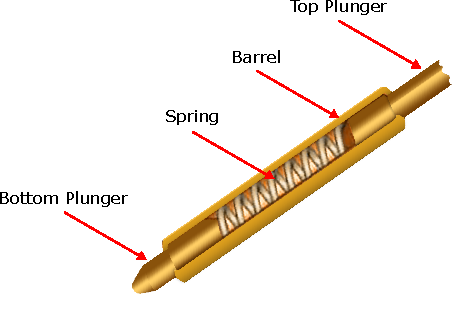
\includegraphics[width=0.72\textwidth]
    {figures/pogo-pin-internals}
    \caption[Internal Structure of a Pogo Pin]{
        An illustration of a typical double-sided pogo pin. The top
        side connects with \acs{IC}'s package, and the bottom side connects with
        exposed copper pads on a PCB.
    }
    \label{fig:pogo-pin-internals}
\end{figure}

Similar to any other conductor, pogo pins suffer from parasitic \ac{RLC}
associated with the overall structure and arrangement of elements in their body.
In addition, the pogo-pin's conductivity is highly dependent on the shape
and amount of contact that plungers or tails at the ends can create when
pressed into the target component pin and \ac{PCB}.
\autoref{fig:pogo-pins-equivalent-circuit} depicts the equivalent circuit of two
pogo pins.

\begin{figure}[h]
    \centering
    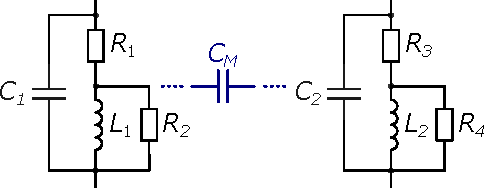
\includegraphics[scale=1.25]
    {figures/pogo-pins-equivalent-circuit}
    \caption[Equivalent Circuit of Pogo Pins]{
        An illustration of a lumped equivalent circuit for pogo pins.
        Each pogo pin has a nominal resistance value ($R_1$, $R_3$), an internal
        inductance ($L_1$, $L_2$) accompanied by a shunt
        resistance ($R_2$, $R_4$)
        and an overall shunt capacitance ($C_1$,$C_2$).
        In addition, a mutual capacitance exists between pogo pins ($C_M$).
    }
    \label{fig:pogo-pins-equivalent-circuit}
\end{figure}

%%%%%%%%%%%%%%%%%%%%%%%%%%%%%%%%%%%%%%%%%%%%%%%%%%%%%%%%%%%%%%%%%%%%%%%%%%%%%%%%

\subsection{Influence of Pogo Pin Shape}
\label{subsec:pogo-pins-shape-influence}
%%%%%%%%%%%%%%%%%%%%%%%%%%%%%%%%%%%%%%%%%%%%%%%%%%%%%%%%%%%%%%%%%%%%%%%%%%%%%%%%

The socket under investigation uses a double-sided pogo pin structure
with crown-shaped plungers on the \ac{DUT} side and cone-shaped plungers on the
load board side as shown in \autoref{fig:pogo-pin-bottom-top}.

\begin{figure}[t]
    \centering
    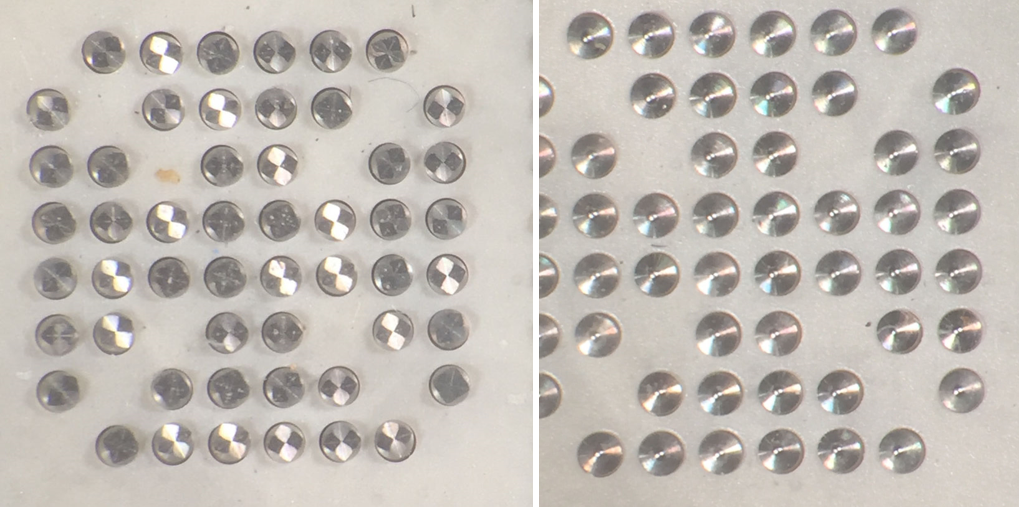
\includegraphics[width=\textwidth]
    {figures/pogo-top-bottom-pins}
    \caption[Double Sided Pogo Socket]{
        The pogo pins of the socket are under investigation. The top pins making
        contact with the \ac{DUT} are crown-shaped (left), and the bottom side
        that makes contact with the load board are cone-shaped (right).
    }
    \label{fig:pogo-pin-bottom-top}
\end{figure}

The socket pogo pins have a sharp center tip at the load board side.
The contact area is less than 20\% of the plunger diameter, and the current
density reaches values beyond
\SI{180}{\ampere\per\milli\meter\squared}.

The large amount of cooling metal behind the tip keeps the overall temperature
low but on a \ac{PCB} with a typical \SI{35}{\micro\meter} copper thickness,
this may result in reliability issues in case of multiple insertions of
\acp{DUT} and closing the socket lid.

Note that the majority of the DC resistance of the pogo comes from internal
wiring (spring) as the pure contact resistance stays in the regime of a few
\SI{}{\milli\ohm} per pogo side.

\autoref{fig:pogo-pin-plunger-bottom} shows the contact form and contact area
on the load board side.
The current density is high although it will not deteriorate the contact
immediately because of the massive cooling behind the tip.
There is a maximum spring force of \SI{0.35}{\newton} which may vary across
the socket, especially after aging.
In that case, we get a non-uniform current distribution across all supply pins
(ground and power), and individual pogo pins may suffer from higher current
density at their contact.

\autoref{fig:pogo-pin-plunger-top} illustrates the top plunger of the pogo pins
where mating between the pogo pin and solder balls of the package is made.
The crown shape of the top plunger provides better contact and increased
reliability against wear-out in comparison to the bottom plunger.

\begin{figure}[h!]
    \centering
    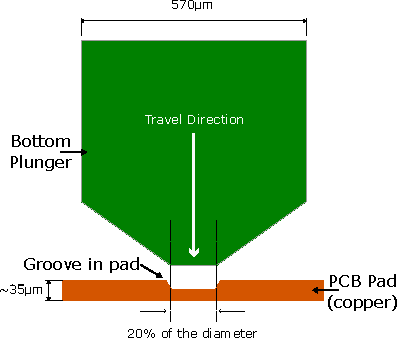
\includegraphics[scale=0.95]
    {figures/pogo_plunger_pcb_connection}
    \caption[Pogo-Pin Plunger connection to PCB Pad]{
        Illustration of pogo pin's bottom side where the connection to a
        \ac{PCB} pad is made.
    }
    \label{fig:pogo-pin-plunger-bottom}
\end{figure}

\begin{figure}[h!]
    \centering
    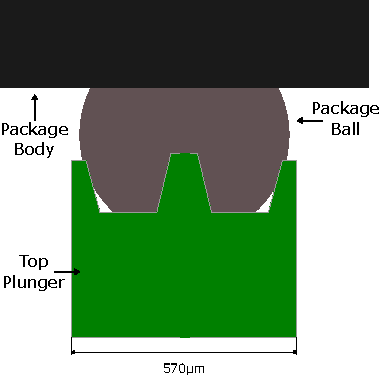
\includegraphics[scale=0.95]
    {figures/pogo_plunger_ball_connection}
    \caption[Pogo-Pin Plunger connection to \acs{DUT}'s Ball]{
        Illustration of pogo pin's top side where the connection to a
        \ac{IC} ball is made.
        The crown tips of the plunger on the top side penetrate the solder
        ball of the chip package and provide a multipoint and secure connection
        to the \acs{DUT}'s solder balls.
    }
    \label{fig:pogo-pin-plunger-top}
\end{figure}

%%%%%%%%%%%%%%%%%%%%%%%%%%%%%%%%%%%%%%%%%%%%%%%%%%%%%%%%%%%%%%%%%%%%%%%%%%%%%%%%

\subsection{Characterization of Pogo Pins}
\label{subsec:characterization-pogo-pins}
%%%%%%%%%%%%%%%%%%%%%%%%%%%%%%%%%%%%%%%%%%%%%%%%%%%%%%%%%%%%%%%%%%%%%%%%%%%%%%%%

All \acp{DUT} are mounted onto the load board using pogo-based sockets.
These sockets have pogo contacts on both sides and a spring for each pogo
inside the socket guarantees proper contact.
The drawback of such a solution is the relatively high resistance of the
contact – the smaller the ball pitch, the higher the pogo resistance.

In order to measure the real resistance of pogo pins, a test setup
concept based on \emph{Kelvin sense} or \emph{four-wire} principle is used
as shown in \autoref{fig:kelvin-measurement-pogo-pin}.
Four-wire measurement significantly reduces the influence of probe leads and wires
by using separate wires for supplying a known test current into the pogo pin and
measuring the voltage drop across a pogo pin under investigation.
\autoref{fig:kelvin-measurement-stand-top} and
\autoref{fig:kelvin-measurement-stand-bottom} shows a set of custom-made probes and
test stand developed to allow
seamless measurement of the socket pins from the top and bottom sides.

\begin{figure}[h!]
    \centering
    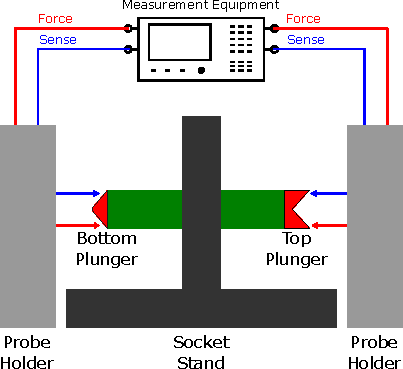
\includegraphics[scale=1.05]
    {figures/kelvin_socket_pogopin_measurement_stand}
    \caption[Kelvin Measurement Stand for Pogo Pins]{
        Kelvin measurement setup for measuring the resistance of pogo pins of
        the socket. Two probe holders were used to fix the tips of kelvin sense
        probes at the bottom and top plungers of pogo pins.
    }
    \label{fig:kelvin-measurement-pogo-pin}
\end{figure}

\begin{figure}[h!]
    \centering
    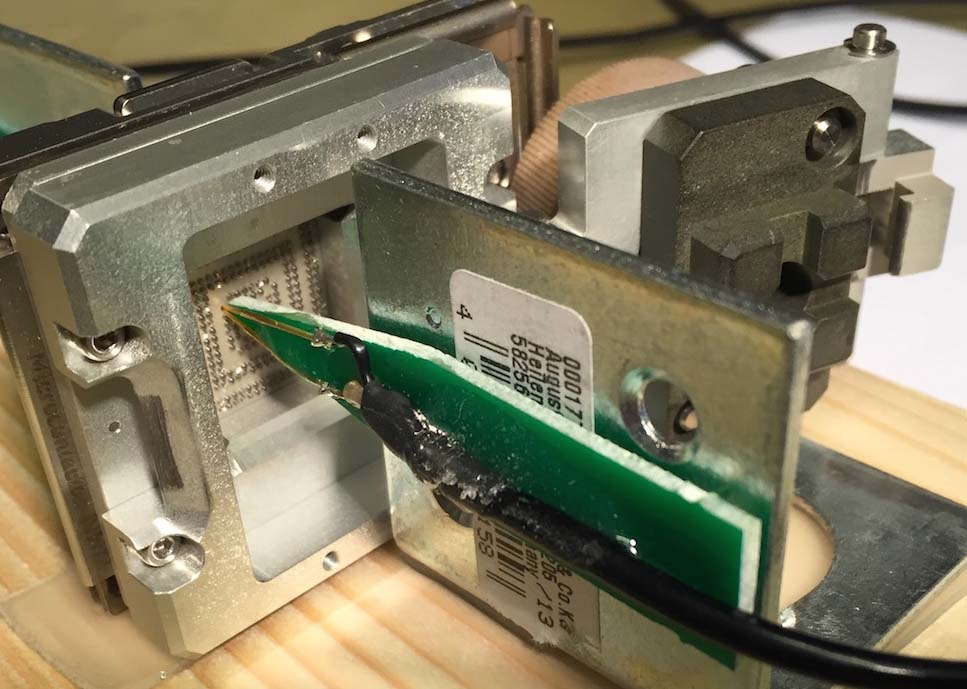
\includegraphics[width=0.8\textwidth]
    {figures/top}
    \caption[Kelvin Measurement Stand Top-Side]{
	The custom-made Kelvin probe is inserted on the top side of the socket.
    }
    \label{fig:kelvin-measurement-stand-top}
\end{figure}

\begin{figure}[h!]
    \centering
    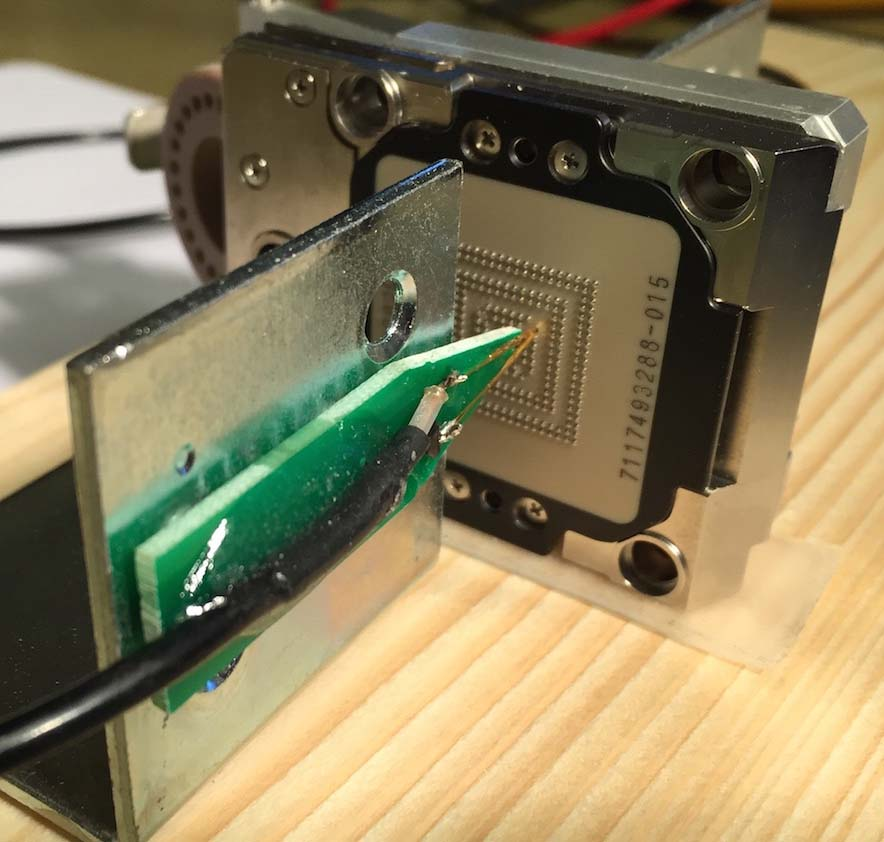
\includegraphics[width=0.8\textwidth]
    {figures/bot}
    \caption[Kelvin Measurement Stand Bottom-Side]{
	Probing the bottom side of the socket using the custom-made Kelvin probe.
    }
    \label{fig:kelvin-measurement-stand-bottom}
\end{figure}

The \acs{DUT}'s \ac{BGA} package gives us a pitch of \SI{0.8}{\milli\meter}, and
the pogo resistance is in the range of \SI{100}{\milli\ohm}.
Datasheets report average values for the resistance at room temperature.
The pogo carry current is reduced by up to $50\%$ at high temperatures as
reported in the datasheet (e.g. from \SI{1}{\ampere} at \SI{23}{\celsius} to
\SI{0.5}{\ampere} at \SI{150}{\celsius}).
It should be noted that the pogo influence depends on the instantiation of the
socket and the parameters may vary per socket due to the manufacturing
tolerances.

Although the pogo inductance of
\SI{0.86}{\nano\henry} sounds low, it
generates slow edges if there is a high demand for current in the nanosecond
regime, and if there is some capacitance on the DUT-internal power and ground
system.
The \acs{DUT}'s internal supply voltage will be delayed by several nanoseconds
if the \acs{DUT} has some ten \SI{}{\pico\farad} of layer capacitance.

%%%%%%%%%%%%%%%%%%%%%%%%%%%%%%%%%%%%%%%%%%%%%%%%%%%%%%%%%%%%%%%%%%%%%%%%%%%%%%%%

\subsection{In-Circuit Socket Evaluation}
\label{subsec:in-circuit-socket-evaluation}
%%%%%%%%%%%%%%%%%%%%%%%%%%%%%%%%%%%%%%%%%%%%%%%%%%%%%%%%%%%%%%%%%%%%%%%%%%%%%%%%

To evaluate the socket in a real-world scenario, a dedicated
evaluation board was developed.
The evaluation board provides access to all major voltage rails and ground
pins of the \ac{DUT} using shielded coaxial cables.
In addition, auxiliary connectors for applying stimulating waveforms (e.g. from
an arbitrary waveform generator) and measuring the results
(e.g. by an oscilloscope) is available on the dedicated evaluation board
\autoref{fig:socket-evaluation-board}.

\begin{figure}[h]
    \centering
    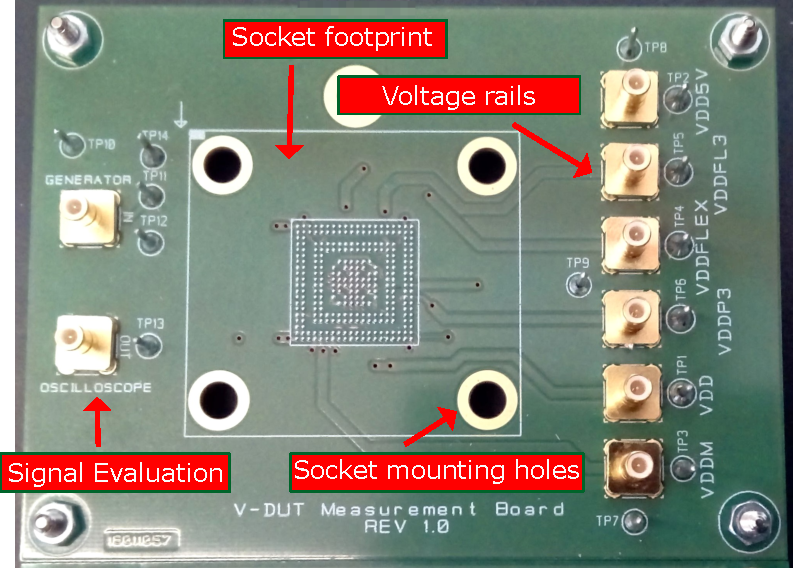
\includegraphics[width=\textwidth]
    {figures/villach-supply-analysis/socket/socket-evalboard}
    \caption[Socket Evaluation Board]{
        Dedicated evaluation board for testing the socket and \acp{DUT}.
        Major voltage rails of the \ac{DUT} are wired to the pins using
        shielded coaxial connectors.
        At the bottom layer, footprints for inserting decoupling capacitors are
        available and can be populated according to the \ac{DUT} recommendation.
    }
    \label{fig:socket-evaluation-board}
\end{figure}

The electrical data of the socket consists of the pogo data and contact quality
on both sides of the socket.
The socket data are available as average values because not all pogo needles are
identical: The pogo resistance varies between \SI{80}{\milli\ohm} at room
temperature and \SI{100}{\milli\ohm} at high temperatures.
Inductance is in the range of \SI{0.9}{\nano\henry}.

The DUT is wired using pogo pins in parallel as shown in
\autoref{fig:pogo-pin-socket-to-dut}, and therefore, the supply
voltages do not drop too far below nominal values:

\begin{figure}[h]
    \centering
    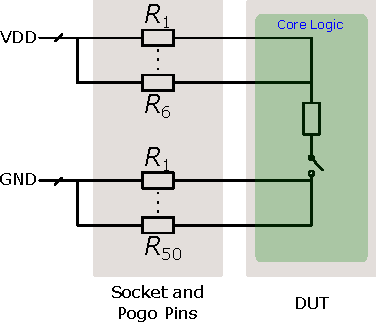
\includegraphics[scale=1.05]
    {figures/pogo-socket-to-dut}
    \caption[Pogo Socket to DUT ]{
        Assigning multiple pins to power and ground is a way to reduce total
        parasitic \acs{RLC} properties. In the case of the \acs{DUT} under
        investigation,
        there are a total of 6 power pins and 50 ground pins in the package.
        The ground pins are scattered around the package and their location is
        based on the internal peripherals of the \acs{DUT}.
    }
    \label{fig:pogo-pin-socket-to-dut}
\end{figure}

\begin{itemize}[topsep=8pt,itemsep=4pt,partopsep=4pt, parsep=4pt]
    \item Digital ground is connected via 50 pogo pins, thus
    reducing interface resistance to a few milliohms.
    \item VDD (digital core supply \SI{1.3}{\volt}) is connected via 6 pogo
    pins.
\end{itemize}

Given a maximum pogo DC resistance of \SI{80}{\milli\ohm}, we get
\SI{13}{\milli\ohm} for the paralleled connection on the high side (6 contacts)
using the custom evaluation board with a \acs{DUT}-sized shorting board as
shown in \autoref{fig:pogo-pin-socket-to-dut} and
\autoref{fig:socket-in-evalboard}, and \SI{2}{\milli\ohm} at GND side
(50 contacts).

For an average core supply current of $I_{DD}=0.55A$ (datasheet for logic
operation) at VDD and a 10\% duty cycle
(\SI{5.5}{\ampere} maximum inrush current) we get a voltage
drop of about \SI{100}{\milli\volt} on high side, and negligible
\SI{11}{\milli\volt} on low side.

\begin{figure}[htbp]
    \centering
    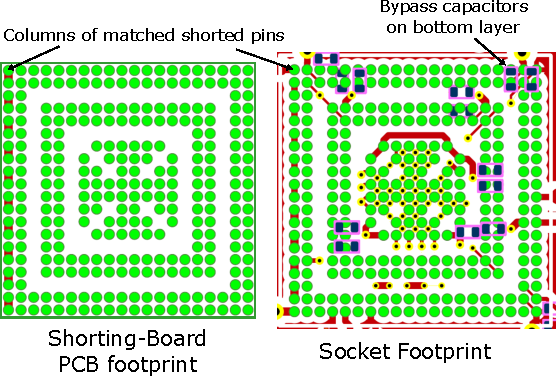
\includegraphics[width=\linewidth,height=0.62\textheight,keepaspectratio]
    {figures/villach-supply-analysis/socket/shorting-dut-pins}
    \caption[DUT For Parallel Pogo Measurement]{
        \textbf{Left:} Top view of the custom \ac{PCB} for parallel measurement
        of socket pins.
        A Row of ground pins are shorted in parallel to measure the
        overall resistance.
        \textbf{Right:} Top view of the socket footprint for the \ac{DUT}.
        Major supply rails and ground are fanned out exactly like the original
        load board.
        On the bottom layer, decoupling capacitors can be soldered to comply with
        datasheet recommendadtion of the \ac{DUT}.
    }
    \label{fig:dut-shorted-pins}
\end{figure}

\begin{figure}[h!]
    \centering
    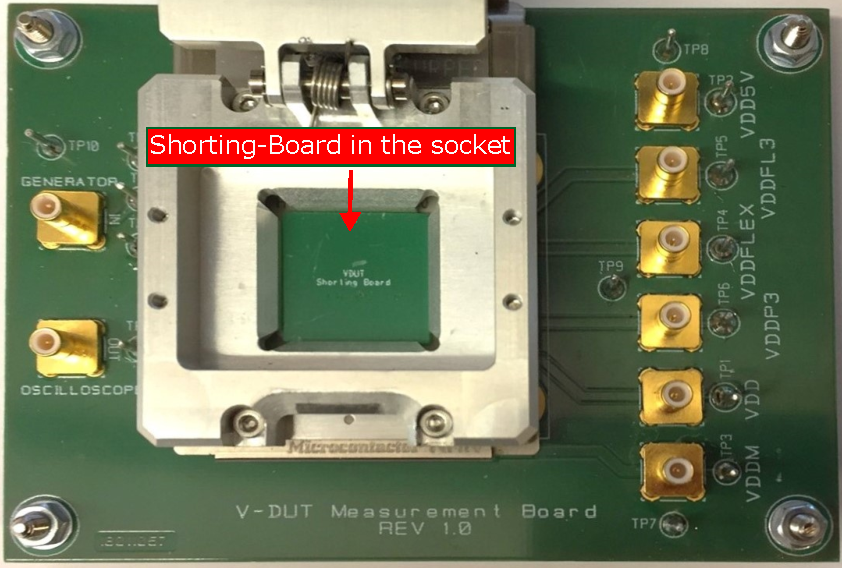
\includegraphics[width=\textwidth]
    {figures/villach-supply-analysis/socket/socket-shorting}
    \caption[Parallel Pogo Measurement]{
        A Socket is installed on the evaluation board and a
        Shorting-Board is inserted into the socket.
        The shorting board shorts a known number of pogo pins in parallel,
        allowing measurement of more than one pogo pin.

    }
    \label{fig:socket-in-evalboard}
\end{figure}

It should be noted that the total drop may vary if the current spike durations
are altered, due to increased temperature and subsequent increase in resistance.
\autoref{table:pogo-pin-vdrop} shows examples of different on-time conditions
(duty cycle) measured with the kelvin sense setup.

\begin{table}[b]
    \centering
    \begin{tabular}{|c|c|c|c|c|}
        \hline
%        \rowcolor[HTML]{FFCCC9}
        \makecell{\textbf{Duty} \\ \textbf{Cycle}} & \makecell{\textbf{V drop} \\ \textbf{PWR Side}} & \makecell{\textbf{V drop} \\ \textbf{GND side}}  & \makecell{\textbf{V drop} \\ \textbf{total}}  & \makecell{\textbf{V DUT @} \\ \textbf{V rail = 1.3V}}  \\ \hline

        20\%  & \SI{46 }{\milli\volt} & \SI{5 }{\milli\volt} & \SI{51 }{\milli\volt} & \SI{1.24}{\volt} \\ \hline
        10\%  & \SI{92 }{\milli\volt} & \SI{11}{\milli\volt} & \SI{102}{\milli\volt} & \SI{1.2 }{\volt} \\ \hline
        5\%  & \SI{183}{\milli\volt} & \SI{22}{\milli\volt} & \SI{205}{\milli\volt} & \SI{1.1 }{\volt} \\ \hline
        2\%  & \SI{458}{\milli\volt} & \SI{55}{\milli\volt} & \SI{513}{\milli\volt} & \SI{0.78}{\volt} \\ \hline

    \end{tabular}
    \caption[Pogo Pin Voltage Drops]{
        Dependence of voltage drop across pogo pin versus maximum current height.
    }
    \label{table:pogo-pin-vdrop}
\end{table}

As stated before, the socket datasheet denotes a significant current reduction at
elevated temperatures so the voltage
drop across the pogo increases if the chip draws equal current at all
temperatures.
This reduces the margins of the supply voltage at high-temperature tests such
that test yield may be influenced.
Measurements performed using the Kelvin test stand have shown that the
resistance of any socket pogo pin increases from an average
of \SI{70}{\milli\ohm} at room temperature to about \SI{90}{\milli\ohm} at
\SI{100}{\celsius}.

It should be noted that the measured values vary slightly with the total travel
of the pogo pin due to changes in length and physical shape of the internal
spring.
Therefore, a dedicated Virtual-\acs{DUT} is necessary to compare individual
current paths.

%%%%%%%%%%%%%%%%%%%%%%%%%%%%%%%%%%%%%%%%%%%%%%%%%%%%%%%%%%%%%%%%%%%%%%%%%%%%%%%%

\subsection{Bandwidth Measurement of the Socket}
\label{subsec:socket-bw-measurement}
%%%%%%%%%%%%%%%%%%%%%%%%%%%%%%%%%%%%%%%%%%%%%%%%%%%%%%%%%%%%%%%%%%%%%%%%%%%%%%%%

The evaluation board is capable of performing bandwidth
and resonance measurements on pogo pins by the addition of \SI{50}{\ohm}
terminated \ac{SMB} connectors for connecting a chain of pogo pins to
a generator and a matching \ac{SMB} connector for acquiring the resulted
waveforms as shown in \autoref{fig:socket-sval-smb-cons}.

\begin{figure}[h!]
    \centering
    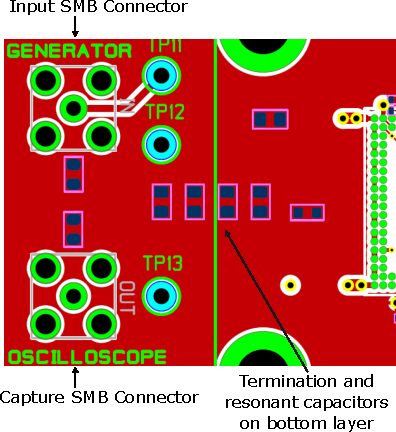
\includegraphics[scale=1.25]
    {figures/villach-supply-analysis/socket/bandwidth-smbs}
    \caption[\acs{SMB} Connectors on Evaluation Board]{
        \ac{SMB} connectors on the left side of the socket evaluation board.
        Termination resistors and resonance capacitors are placed on the bottom
        layer.
    }
    \label{fig:socket-sval-smb-cons}
\end{figure}

The evaluation board can be setup for measuring series resonance and
bandwidth of a chain of pogo pins according to
\autoref{fig:socket-setup-bw-meas} and
\autoref{fig:socket-setup-resonance-meas}.

\begin{figure}[htbp]
    \centering
    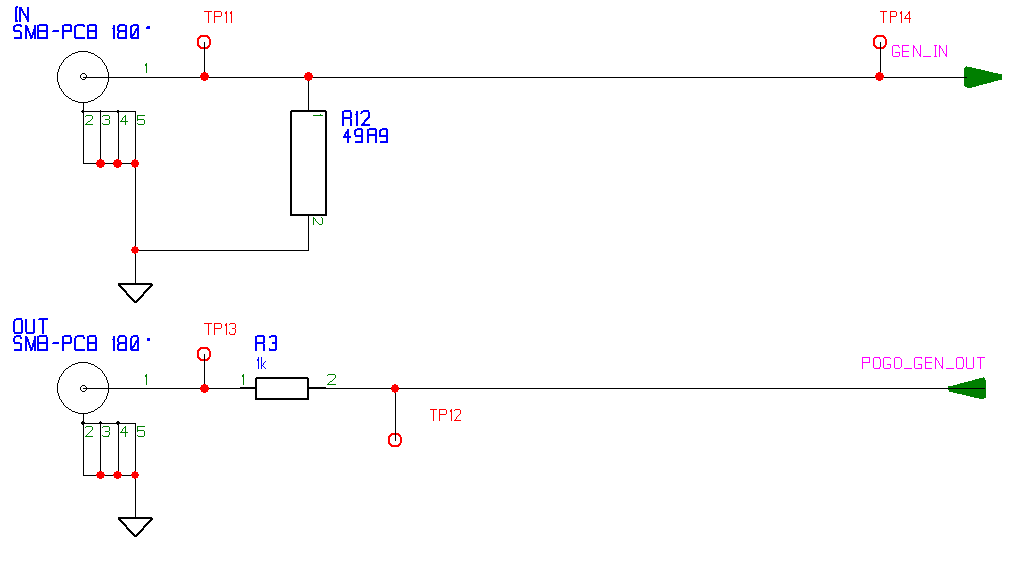
\includegraphics[width=\linewidth,height=0.62\textheight,keepaspectratio]
    {figures/villach-supply-analysis/socket/image29}
    \caption[Socket B/W Measurement Setup]{
        Socket evaluation board setup for \emph{Socket Bandwidth} measurement
        (transversal mode).
    }
    \label{fig:socket-setup-bw-meas}
\end{figure}

\begin{figure}[htbp]
    \centering
    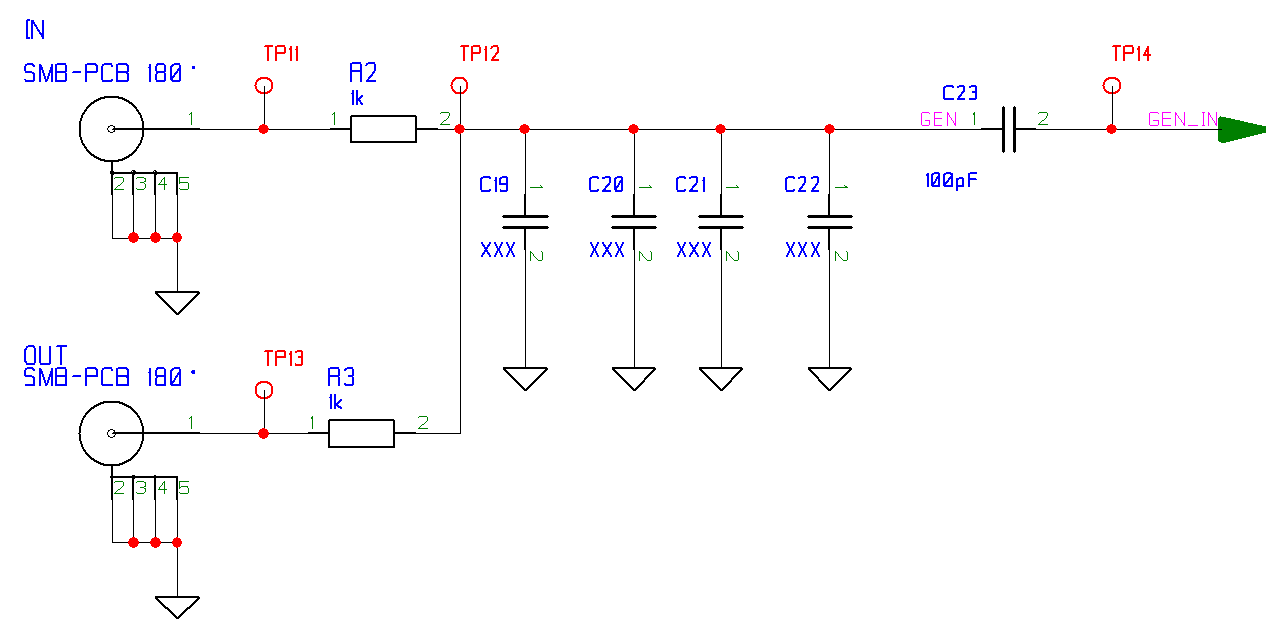
\includegraphics[width=\linewidth,height=0.62\textheight,keepaspectratio]
    {figures/villach-supply-analysis/socket/image30}
    \caption[Socket Resonance Measurement Setup]{
        Socket evaluation board setup for \emph{Socket Resonance} measurement
        (series resonance mode).
        Placeholders for capacitors and resistors are available to be populated
        by exact values to create an L/C Tank circuit.
    }
    \label{fig:socket-setup-resonance-meas}
\end{figure}

The shorting board is then stimulated with a sinusoidal function from an
\acs{RF} signal generator and the response was captured by a network analyzer
with an equivalent setup depicted in
\autoref{fig:bw-meas-equivalent-circuit}.
After applying a test waveform through 20 pogo pins in series, the resulting
waveform was captured as presented in \autoref{fig:bw-meas-result}.

\begin{figure}[htbp]
    \centering
    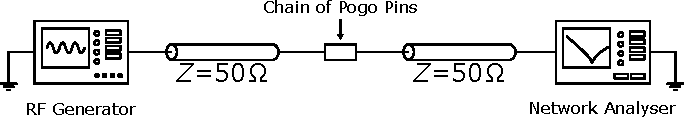
\includegraphics[width=\linewidth,height=0.62\textheight,keepaspectratio]
    {figures/villach-supply-analysis/socket/bw-meas-equivalent-circuit}
    \caption[Equivalent Circuit for Socket B/W Measurement]{
        Equivalent circuit for bandwidth measurement of a chain of pogo pins.
    }
    \label{fig:bw-meas-equivalent-circuit}
\end{figure}

\begin{figure}[h!]
    \centering
    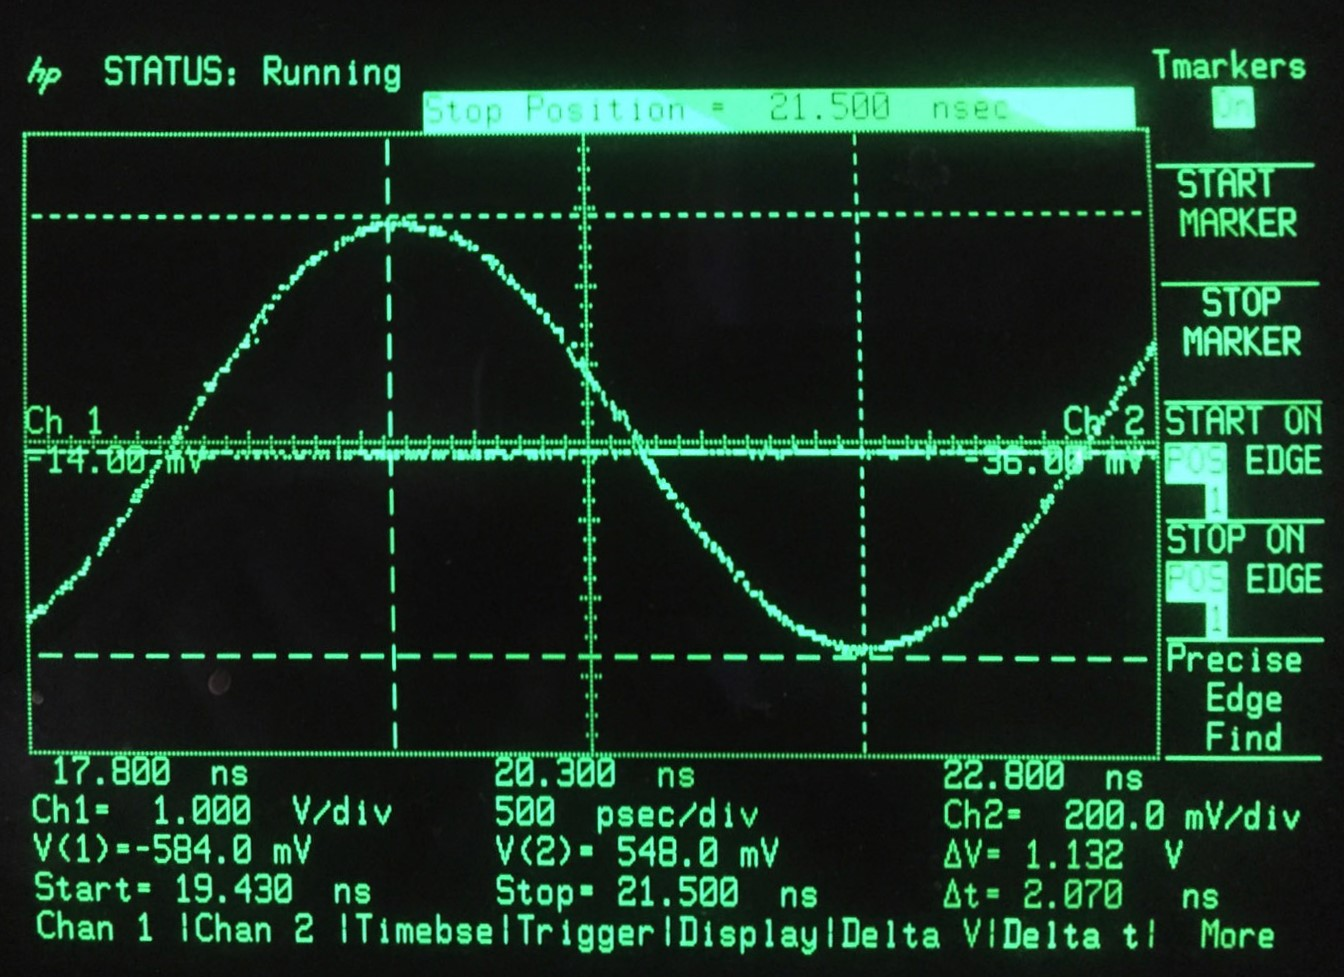
\includegraphics[width=\textwidth]
    {figures/villach-supply-analysis/socket/bw-result}
    \caption[Result of Socket B/W Measurement]{
        Signal waveform after passing through 20 pogo pins inside the socket.
        The 100\% signal height is at \SI{250}{\mega\hertz}.
    }
    \label{fig:bw-meas-result}
\end{figure}

The measured \SI{3}{\decibel} bandwidth
for a chain of 20 pogo pins is \SI{550}{\mega\hertz} and exceeds the
capabilities of the load board bandwidth.
Therefore, the socket is well-suited for high-speed applications.

By configuring the socket evaluation board as an \emph{LC Tank} circuit
according to \autoref{fig:inductance-meas-equiv}, a known capacitor value
can solve for an unknown inductor (chain of pogo pins in this case) according to
\autoref{eq:resonant-freq}.

\begin{figure}[htbp]
    \centering
    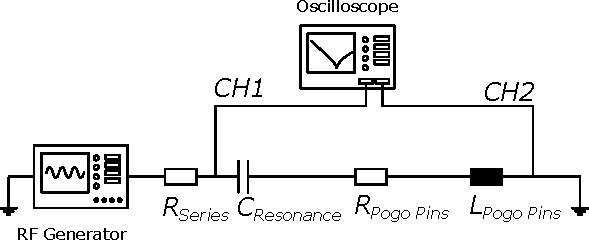
\includegraphics[width=\linewidth,height=0.62\textheight,keepaspectratio]
    {figures/villach-supply-analysis/socket/resonance-meas-circuit}
    \caption[Equivalent Circuit for Inductance Measurement]{
        Equivalent circuit of the inductance measurement using \emph{LC Tank}
        circuit.
        $R_{series}$ is added for controlled damping by adjusting
        $Q$ (quality factor) and impedance matching purposes.
    }
    \label{fig:inductance-meas-equiv}
\end{figure}

\begin{equation}
    \label{eq:resonant-freq}
    f_0 = \frac{1}{2\pi\sqrt{LC}}
\end{equation}

The \emph{LC Tank} equipped with a \SI{100}{\pico\farad} capacitor
exhibits a \SI{500}{\mega\hertz} resonance frequency, leading to an inductance
value of \SI{1}{\nano\henry} which is very close to the datasheet reported
value of \SI{0.8}{\nano\henry}.

%%%%%%%%%%%%%%%%%%%%%%%%%%%%%%%%%%%%%%%%%%%%%%%%%%%%%%%%%%%%%%%%%%%%%%%%%%%%%%%%

\subsection{Summary of Socket Evaluation}
\label{subsec:summary-socket-evaluation}
%%%%%%%%%%%%%%%%%%%%%%%%%%%%%%%%%%%%%%%%%%%%%%%%%%%%%%%%%%%%%%%%%%%%%%%%%%%%%%%%

The measurements on the socket show that the most important influence of
the socket is its resistance when it comes to large current spikes like
in SCAN test.
Whereas socket resistance is critical, no limitations regarding the
socket bandwidth is observed – i.e. socket inductance and socket capacitance do
not contribute significantly to bandwidth limitations.
The disturbing influence of the socket comes from the voltage drop during
fast current waveforms when all digital components switch inside the DUT
at the time of the clock edge.

A precise DUT model is necessary to get precise simulation results and the
inductive influence cannot be judged without knowing the chip-internal layout.
There are power supply planes, and their connections to the balls will lead to
a current distribution that may alter core supply voltages to some extent:

\begin{itemize}[topsep=8pt,itemsep=4pt,partopsep=4pt, parsep=4pt]

    \item
    The pogo inductance shifts the voltage rise for a maximum
    of \SI{10}{\nano\second}, i.e. there may be a slight timing difference for
    individual logic core blocks if the internal power distribution
    is segmented.

    \item
    The start-up and shutdown phases of the DPS supplies are not tangled by the
    inductance.
    It is the operational DUT supply current during current-intensive tests
    like SCAN where the speed of the device components dictates the rise and
    fall of the supply currents. The inductive influence puts a burden
    on the supply quality if there are other issues that reduce overall
    rail quality (if we do not clock the DUT fast, the time shift in core rails
    will most probably be acceptable).

\end{itemize}

The following list summarizes the findings regarding voltage drop
due to parasitic characteristics exhibited by the socket and pogo-pins:

\begin{enumerate}[topsep=8pt,itemsep=4pt,partopsep=4pt, parsep=4pt]

    \item
    The supply voltage for the \acs{DUT} core should be increased slightly to
    compensate for the drop.

    \item
    There should be large support capacitors (blocking caps) even if the
    \acs{ATE}'s \ac{DPS} reacts with overshoot.
    In a worst-case scenario, we should increase the voltage step-wise to avoid
    development of overshoot at the \ac{DUT} site.

    \item
    The inductance of the pogo cannot be reduced because it depends on the basic
    construction of the contact form.
    Therefore, power-hungry high-current tests should not be run at high
    tester speed to allow for rail settling before testing by reducing scan test
    clock rate to lower values.
    It should be detectable when the clock is beyond reliable values if
    test yield drops sharply.

    \item
    The contact resistance depends on the force under which
    the DUT is pressed onto the pogo pins. Because there is a statistical
    distribution of spring force we may get different resistance values for
    different pogo pins in an array.

    \item
    Contact wear-out of the pogo pins can play a role in measurement
    results. Every \ac{DUT} insertion and extraction cycle reduces the
    sharpness of the pogo pins, resulting in higher resistance values over time.

\end{enumerate}



